
% this file is called up by thesis.tex
% content in this file will be fed into the main document

%: ----------------------- introduction file header -----------------------
\begin{savequote}[50mm]
Historical methodology, as I see it, is a product of common sense applied to circumstances. 
\qauthor{Samuel E. Morison}
\end{savequote}


\chapter{Método para la evaluación de competencias genéricas}
\label{cha:Overall methodology}

% the code below specifies where the figures are stored
\ifpdf
    \graphicspath{{4_overall_methodology/figures/PNG/}{4_overall_methodology/figures/PDF/}{4_overall_methodology/figures/}}
\else
    \graphicspath{{4_overall_methodology/figures/EPS/}{4_overall_methodology/figures/}}
\fi

%------------------------------------------------------------------------- 

En este capítulo se propone un método para la evaluación de competencias genéricas de los estudiantes basado en el diseño de evaluaciones a partir de la actividad de estos en los entornos de aprendizaje. El capítulo comienza con una introducción; en segundo lugar, se presenta una descripción detallada del método. Y en tercer lugar, se demuestra como el método satisface las características de una propuesta basada en el diseño (DBR), se describen los requisitos que el método ha de satisfacer y se introduce el tipo de herramienta que se empleará para su implementación.

\section{Introducción}

Se podría decir que hoy en día los entornos virtuales constituyen una pieza fundamental en cualquier contexto en el que se impartan cursos. Mientras que en los cursos virtuales, los VLEs son el único entorno de trabajo posible, en los cursos presenciales, tantos los VLEs como otras herramientas virtuales actúan como soporte virtual de las clases, proporcionando multitud de actividades de aprendizaje. 

En el VLE por ejemplo, los estudiantes pasan a diario por sus páginas. Por un lado, habrá estudiantes que entren en el VLE varias veces al día a consultar cualquier novedad y que sólo permanezcan 20 segundos en el mismo. Mientras que por otro lado, habrá estudiantes que entren una vez a la semana pero estén dos horas navegando por el VLE. Y entre un tipo de estudiante y otro, habrá tantas maneras de actuar de los estudiantes en el VLE como estudiantes haya. 

Todas las acciones de los estudiantes quedan almacenadas en el registro de las actividades de aprendizaje, y estos registros podrían ser analizados para comprender el proceso de aprendizaje que se está desarrollando. %El \emph{learning analytics} es un área de investigación del aprendizaje mejorado por la tecnología (TEL, del inglés \emph{Technology Enhanced Learning}) que está enfocado en el desarrollo de métodos para analizar y detectar patrones en los datos recogidos en los entornos educativos y aprovecharlos para mejorar el aprendizaje~\cite{chatti2014learning}.

En esta tesis se propone un método de evaluación de competencias genéricas basado en el diseño de evaluaciones (DBA, del inglés, \emph{design-based assessment}) y que tiene su origen en la investigación basada en el diseño (DBR). DBA es un método de evaluación de competencias genéricas que se basa en indicadores de la actividad generada por los estudiantes en los entornos de aprendizaje virtual. Los profesores podrán diseñar evaluaciones utilizando estos indicadores y podrán utilizar estas evaluaciones como evidencias del desempeño de competencias genéricas. Estas evaluaciones podrán ser refinadas por el propio profesor hasta llegar a unas evidencias que le sean válidas. También podrán ser utilizadas y modificadas por otros profesores que busquen adaptarlo a su contexto local o a las competencias que ellos quieren realizar. 

% ---- Comentarios ----------
% Hay que hablar en capítulos anteriores de registros en actividades de aprendizaje y no en el VLE
% Porque aquí las actividades de aprendizaje son 3: wiki, VLE y WV.


\section{Método: design-based assessment (DBA)}

\subsection{Contexto}

Los estudiantes comienzan a dejar constancia de su actividad en los entornos virtuales desde el momento en que acceden al entorno. El registro del sistema lo almacena todo, tanto la participación activa del estudiante, escribiendo y respondiendo mensajes en los foros o enviando actividades, como la participación pasiva, cuando simplemente se lee una página, se leen los mensajes del foro o se descargan los apuntes. 

Los programas de las asignaturas incluyen las competencias genéricas de las que los estudiantes deben ser evaluados. Los profesores pueden plantear actividades en los entornos virtuales con la intención no sólo de evaluar ciertas habilidades de los estudiantes, sino también de provocar comportamientos en los estudiantes y ver cómo afrontan ciertas situaciones. Pueden encontrarse patrones de comportamiento en la manera en que los estudiantes abordan ciertas tareas y estos comportamientos podrían ser interpretados como un indicador del desempeño de alguna competencia genérica.

Para evaluar una competencia genérica dada, el profesor podrá diseñar una evaluación a partir de la información relativa a los registros de los entornos de aprendizaje. Aquí comienza un \emph{ciclo de contraste de hipótesis}. 

%Ese diseño será procesado por el sistema que implementa el método y que terminará devolviendo la información al profesor. El resultado de aplicar el diseño será un indicador que el profesor podrá utilizar para la evaluación de la competencia genérica.


%También se puede dar el caso de que el profesor considere que el indicador no es válido para la evaluación de la competencia genérica. También puede que aunque le sea válido pero considere que un rediseño del mismo le permitirá afinar más en cuánto al objetivo de evaluación de competencia genérica que se marcó. El profesor podría diseñar una nueva evaluación a partir de la información contenida en el registro y así sucesivamente hasta que los resultados satisfagan su hipótesis, momento en el que termina el  \emph{ciclo de contraste de hipótesis}.


\subsection{Descripción del método}

El método DBA es iterativo, ya que permite al docente rediseñar y contrastar hipótesis y resultados hasta confirmar la hipótesis, o por el contrario, descartarla y enunciar una nueva. Podemos decir que el método se integra en un \emph{ciclo de contraste de hipótesis}. Este ciclo consta de una serie de pasos que se muestran en la figura~\ref{fig:CCHDiagram} y se explican a continuación:

\begin{figure}
  \begin{center}
    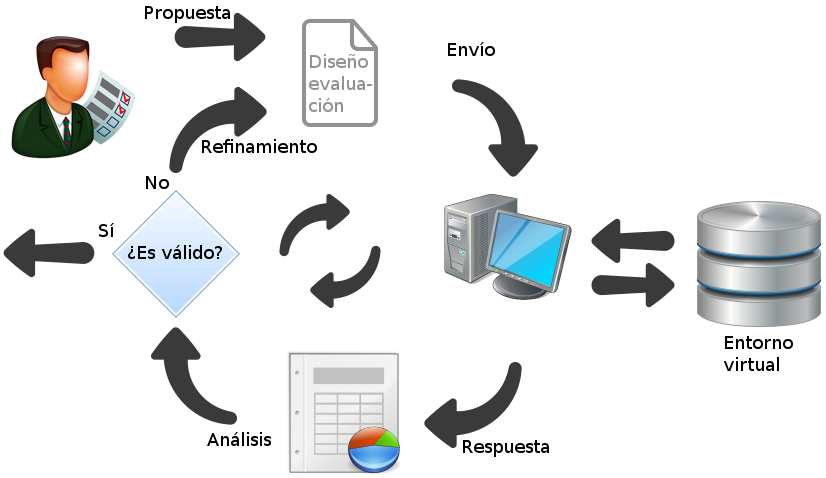
\includegraphics[scale=0.45]{CCHDiagram.png}
  \end{center}
  \caption{Diagrama del ciclo de contraste de hipótesis}
  \label{fig:CCHDiagram}
\end{figure}

\begin{enumerate}
\item \emph{Hipótesis inicial}: el profesor formula una hipótesis para la utilización de algún tipo de información de la actividad de los estudiantes en el entorno virtual para la evaluación de alguna competencia genérica (a). Por ejemplo, se considerará que un estudiante tiene un desempeño correcto de la competencia genérica de planificación y gestión del tiempo si entrega las tareas programadas por el profesor en el VLE con anterioridad a la fecha fijada para las mismas.
\item \emph{Diseño y formulación de evaluación}: el profesor diseñará un indicador para evaluar la competencia a partir de la información del registro y la implementará en la herramienta utilizada para extraer la información (b). Por ejemplo, podríamos considerar partiendo de la hipótesis anterior que un estudiante tendrá un desempeño alto en la competencia de planificación y gestión del tiempo si de las 10 tareas programadas durante el semestre al menos 9 fueron entregadas antes de la fecha fijada para las mismas, un desempeño medio si entregó entre 7 y 8 tareas antes de la fecha fijada y un desempeño bajo si entregó 6 o menos tareas antes de la fecha fijada.
\item \emph{Petición de datos}: Se enviará la petición de datos al sistema encargado de recuperar la información (c). Las herramientas y su funcionamiento serán explicadas más adelante en la sección~\ref{sec:tools}.
\item \emph{Validación de resultados}: la herramienta pondrá a disposición del profesor los indicadores requeridos (d). El profesor los analizará (e) y evaluará si son válidos para el propósito que fueron diseñados (f), si necesitan ser refinados o si hay que descartarlos. En este caso, podrá volver al segundo punto y rediseñar una nueva evaluación (g).
\end{enumerate}

\section{Características, requisitos y herramienta}

El método DBA para la evaluación de competencias genéricas es un método DBR. Aunque desde el punto de vista del estudiante y considerando la clasificación de métodos de evaluación mostrada en la sección~\ref{sec:methods} diríamos que es un método \emph{evaluación formativo}, ya que permite mejorar el aprendizaje mientras este tiene lugar proporcionando información de manera sistemática y continua. Sin embargo, lo consideramos un método DBR ya que no mejora únicamente la acción del alumno, sino que también es un método de investigación que mejora la acción del profesor.

Mientras que con respecto a la clasificación de técnicas de evaluación mostrada en la sección~\ref{sec:techniques}, la técnica empleada en este método es la de obtención de \emph{indicadores del trabajo en actividades de aprendizaje}.

\subsection{Características}

En el apartado~\ref{sec:dbr} se indican, partiendo del análisis realizado por Terry Andersen y Julie Shattuck~\cite{anderson2012design}, las características que un estudio DBR de calidad debe tener. A continuación se identificará nuestro método DBA en cada una de esas características:

\begin{itemize}
\item \emph{Estar situado en un contexto educativo real}: el método DBA se puede utilizar en contextos educativos reales. De hecho, el método ya ha sido utilizado en diferentes asignaturas de la Universidad de Cádiz y los resultados de la investigación han sido publicados en revistas y congresos del área de las TEL~\cite{Balderas:2012,Balderas:2013,balderas2013generative,Balderas:2015,balderas2015domain}.
\item \emph{Enfocado en el diseño y prueba de una intervención significativa}: La intervención que se lleva a cabo con el método DBA es un \emph{tipo de evaluación}, siendo este uno de los tipos de intervenciones recogidos en la tipología de intervenciones DBR definida por Andersen~\cite{anderson2012design}. 
\item \emph{Empleo de métodos mixtos}: una intervención DBR implica normalmente la aplicación de diferentes métodos, técnicas y herramientas. El método DBA puede combinarse con otros métodos de evaluación con el fin de contrastar evaluaciones y dar validez a los resultados obtenidos con uno u otro método.
\item \emph{Múltiples iteraciones}: el método DBA permite el diseño de evaluaciones y su contraste de resultados (\emph{ciclo de contraste de hipótesis}). A partir de los resultados, el diseño se puede ir refinando iterativamente hasta que los resultados satisfagan las expectativas del profesor o hasta que decida descartarlos por no ser válidos para su evaluación.
\item \emph{Asociación colaborativa entre investigadores y profesores}: el método DBA permite la colaboración entre los investigadores, personal con perfil tecnológico del área de la informática, y profesores sin perfil tecnológico de cualquier área. Para ello, se implementa una herramienta que permita aplicar el método a profesores sin conocimientos técnicos, y así tanto investigadores como profesores pueden poner en común su experiencia y los resultados que van obteniendo.
\item \emph{Evolución de los principios de diseño}: el método DBA permite la creación de diseños para aplicar a diferentes competencias. Ciertos diseños podrían ser definidos como plantillas o patrones para la evaluación de competencias. Estos patrones podrán ser utilizados por otros profesores, y a partir de su reflexión, modificados para ser adaptados a nuevos contextos. De esta forma, los principios y diseños creados por profesores e investigadores no mueren con una práctica, sino que son puntos de partidas para nuevas teorías y experimentos.
\item \emph{Comparación con la investigación-acción}: El objetivo del método DBA, al contrario de lo que ocurre con la investigación-acción, no es sólo alcanzar una serie de objetivos a nivel local, sino que también permite evolucionar a nivel teórico y maximizar la generalización, mejorando así la comprensión de aplicaciones prácticas. Además, permite la participación de un equipo formado por investigadores y profesores.
\item \emph{Repercusión en las prácticas}: El método DBA puede repercutir directamente en las prácticas. A partir de su aplicación en las sesiones prácticas y del análisis de resultados, los investigadores y profesores implicados pueden detectar actividades e interacciones que favorecen el desempeño de competencias y que no habían considerado anteriormente. Esto repercutirá directamente en la organización y programación de actividades en los siguientes cursos.
\end{itemize}

\subsection{Requisitos}

El método debe cumplir una serie de requisitos que parten de los inconvenientes encontrados en la revisión de la literatura realizada en el capítulo \ref{cha:State of the Art} y que han sido resumidos en el capítulo \ref{cha:Problemas}. A continuación se describe cada uno de estos requisitos.

\paragraph*{1. Indicadores objetivos}

Los indicadores reflejan los datos obtenidos directamente del registro de las actividades de aprendizaje, por lo que serán objetivos per sé. No ha lugar a consideraciones personales o interpretaciones inexactas de rúbricas cómo ocurría en la autoevaluación o evaluación entre iguales, dónde dos evaluaciones de un mismo trabajo realizadas por personas diferentes podrían tener calificaciones diferentes. En el caso de los indicadores obtenidos del registro de las actividades aprendizaje, dos estudiantes que tienen los mismos datos en el registro tendrán en el mismo valor en el indicador, y ya será decisión del profesor la interpretación del indicador.

\paragraph*{2. Evaluación escalable}

El método para la evaluación de competencias genéricas es escalable y no supone al profesor un esfuerzo que éste no pueda abordar. El método se implementa en una herramienta que se alinea con las actividades aprendizaje. El profesor puede consultar los indicadores del registro con una simple petición a la herramienta. Entonces, esta procesa la petición y la información es devuelta en formatos que el profesor puede visionar y exportar a otras herramientas.

\paragraph*{3. Propósito general}

El propósito del método es obtener indicadores del registro de las actividades de aprendizaje y que estos sean utilizados para evaluar competencias genéricas. Pero no están orientados a una competencia genérica concreta, sino que es el profesor quien diseña sus actividades en el entorno virtual y el que luego obtiene los indicadores para después utilizarlos en la evaluación de la competencia genérica que considera que los estudiantes han desempeñado en dicha tarea (y que queda reflejada en los indicadores). El profesor podría incluso utilizar los indicadores para evaluar competencias específicas si lo creyese oportuno. Pero en ningún caso este método tiene como propósito una competencia y actividad concreta como ocurría, por ejemplo, con algunos juegos serios recogidos en el estado del arte.

\paragraph*{4. Accesibilidad}

No es necesario que el profesor tenga un perfil informático u otro específico para poder realizar las peticiones de los indicadores, ni que contrate a un equipo de expertos para obtener los indicadores. La interfaz en la que se implementa el método es usable y sencilla para que los profesores puedan utilizarla sin requerirles conocimientos técnicos, y los formatos a los que se exporta la información son figuras y documentos en formatos transportables a cualquier hoja de cálculo.

\paragraph*{5. Diseño de evaluaciones}

La herramienta proporciona al profesor la posibilidad de diseñar sus propias evaluaciones a partir de los indicadores. En el estado del arte nos encontramos con trabajos que obtenían sus evaluaciones a partir de los indicadores del VLE, pero éstos eran fijos. Es decir, cada competencia se evaluaba con un indicador dado. Pero podía ocurrir que el profesor no utilizase las actividades del VLE que proporcionaban dichos indicadores o que plantease las actividades con un enfoque diferente al que realmente tienen. Por ejemplo, uno de los puntos fuertes de un wiki es que favorecen el trabajo colaborativo, y podríamos encontrar herramientas que nos ayuden a valorar el trabajo en equipo de los estudiantes que participan en una página de un wiki mediante indicadores del trabajo colaborativo. Si un profesor plantea actividades en el wiki de manera que cada estudiante trabaje individualmente en una página, podrá valorar otras competencias, pero el trabajo en equipo no. Con este método el profesor es quién diseña sus indicadores, y por tanto, sus evaluaciones a partir de los registros de las actividades de aprendizaje.

En resumen, podemos decir que el método que se propone para evaluar competencias genéricas a partir de los registros de interacción de las actividades de aprendizaje se pone a disposición del profesor en forma de una herramienta informática que se conecta a la actividad de aprendizaje utilizado en la asignatura. Mediante esta herramienta, los profesores pueden diseñar evaluaciones a partir de indicadores objetivos obtenidos del VLE y aplicarlos a las competencias genéricas para las que ellos consideren que les son válidos.

\subsection{Herramienta}

La herramienta que implemente el método debe cumplir una serie de requisitos que ayuden a alcanzar los mencionados en el punto anterior:

\begin{itemize}
\item \emph{Cercana al dominio}: la herramienta debe servir al profesor o investigador para definir indicadores a partir de la actividad de los estudiantes en los entornos de aprendizaje, por tanto, debe ser una herramienta definida en términos del ámbito educativo.
\item \emph{Personalización de evaluaciones}: la herramienta debe proporcionar un mecanismo para permitir al usuario crear sus diseños a partir de los indicadores disponibles en el entorno virtual.
\item \emph{Usabilidad}: la herramienta debe ser usable por usuarios de perfil no informático, por lo que su utilización debe ser sencilla y entendible por este tipo de usuarios.
\end{itemize}

A tenor de estos requisitos se decidió que la herramienta informática a implementar sería un \emph{lenguaje específico de dominio} (\emph{DSL}, del inglés, \emph{domain-specific language}). Un DSL es un lenguaje de programación orientado a un dominio concreto. Estos se han vuelto muy populares en los últimos años, y una de las principales razones es que facilitan la comunicación con los expertos en el dominio, proporcionando un texto común (código escrito en el DSL) que actúa a la vez como ejecutable y como una descripción que los expertos en el dominio pueden leer para entender como sus ideas se representan en el sistema~\cite{fowler2010domain}. En el método DBA, el ejecutable seria el diseño y los expertos en el dominio los profesores.



% La evaluación de las 3 herramientas se corresponde al capítulo siguiente.


%Metodología mixta

%Cómo voy a evaluar roles, momentos, actividad, ... lo que sea.

%Explicar el DSL

%DSL: herramienta de investigación en evaluaciones. Esta herramienta ayuda al investigador a formalizar la evaluación.
 
%Enfocar la metodología a que no es una metodología para evaluar, sino para diseñar evaluaciones. Diseñador de evaluaciones.

%Explicar qué pasos tiene que seguir un diseñador de evaluaciones para hacer sus evaluaciones.

%Dentro de los resultados obtenemos dos cosas:
%1. Diseño
%2. Lo que el diseñador nos indicó que no pudo hacer

%Para que esto sea posible falta la herramienta informática

%\section{Evolución herramientas}

%AMW --> EvalCourse --> EvalSim

%\section{Metodología de desarrollo}

%DSL? Ing. Dirigida x modelo?



%------------------------------------------------------------------------------------------------------------------------------------------------

